\documentclass[../entwurf.tex]{subfiles}
\begin{document}

\section{StepDetection-Library}
    \subsection{Input}
        \sign{public class Input : IObservable<AccGyroData>}
        
        \begin{center}
            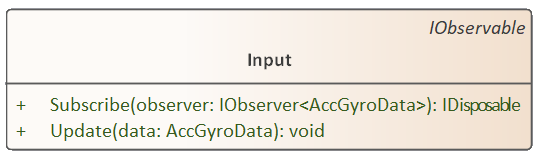
\includegraphics[scale=0.75]{../uml_klassen/StepDetectionLib/Input.png}
        \end{center}
        Nimmt Beschleuninigunsdaten entgegen und gibt diese an Beobachter als struct AccGyroData weiter.
        \paragraph{Methoden}
        \begin{itemize}
            \i{public IDisposable Subscribe(IObserver<AccGyroData> observer)} Fügt neue Beobachter hinzu.
            \i{public void Update(AccGyroData data)} Pusht Daten zu den Beobachtern.
            \i{public void ValueChanged(object sender, EventArgs args)} Nimmt Beschleuninigunsdaten entgegen.
        \end{itemize}


    \subsection{AccGyroData}
    \sign{public struct AccGyroData}
    	
    	\begin{minipage}{0.4\textwidth}
    		 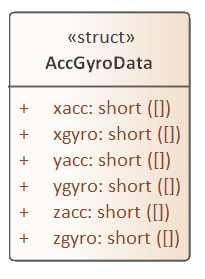
\includegraphics[scale=0.75]{../uml_klassen/StepDetectionLib/AccGyroData.png}
    	\end{minipage}
    	\begin{minipage}{0.6\textwidth}
    		
        	Enthält Beschleuninigunsdaten.
    	\end{minipage}
        \paragraph{Properties:}
        \begin{itemize}
            \i{public short[] xacc} Beschleuninigunsdaten x-Achse.
            \i{public short[] yacc} Beschleuninigunsdaten y-Achse.
            \i{public short[] zacc} Beschleuninigunsdaten z-Achse.
            \i{public short[] xgyro} Beschleuninigunsdaten x-Drehung.
            \i{public short[] ygyro} Beschleuninigunsdaten y-Drehung.
            \i{public short[] zgyro} Beschleuninigunsdaten z-Drehung.
        \end{itemize}

    \subsection{StepDetectionAlg}
    \sign{class StepDetectionAlg :IObserver<AccGyroData>, 	IObservable<Output>}
    	
    	\begin{minipage}{0.75\textwidth}
    		 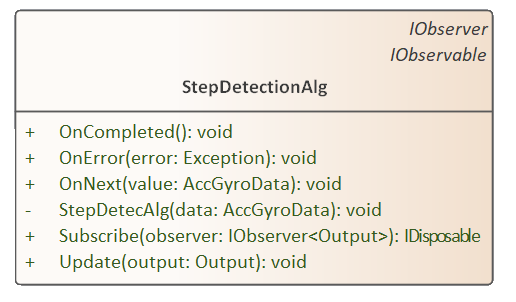
\includegraphics[scale=0.75]{../uml_klassen/StepDetectionLib/StepDetectionAlg.png}
    	\end{minipage}
    	\begin{minipage}{0.25\textwidth}
    		
        Erhält struct AccGyroData von Input und berechnet anhand der Daten Schrittfrequenz und Anzahl der Schritte
    	\end{minipage}
        \paragraph{Properties:}
        \begin{itemize}
            \i{private List<IObserver<Output>> observers} Liste mit Beobachtern.
        \end{itemize}
    
        \paragraph{Methoden}
        \begin{itemize}
            \i{public void OnCompleted()} Wenn Subjekt fertig mit der Datenübertragung ist.
            \i{public void OnError(Exception error)} Wenn Subject einen Fehler erfährt.
            \i{public void OnNext(AccGyroData value)} Enthält Daten von Subjekt.
            \i{public IDisposable Subscribe(IObserver<Output> observer)} Fügt neue Beobachter hinzu.
            \i{public void Update(Output output)} Pusht Daten zu Beobachtern.
            \i{private void StepDetecAlg(AccGyroData data)} Berechnet Schrittfrequenz und Anzahl der Schritte.
        \end{itemize}
    
    \subsection{Outputmanager}
    \sign{public class OutputManager : IObservable<Output>, IObserver<Output>}
    	\begin{minipage}{0.75\textwidth}
    		  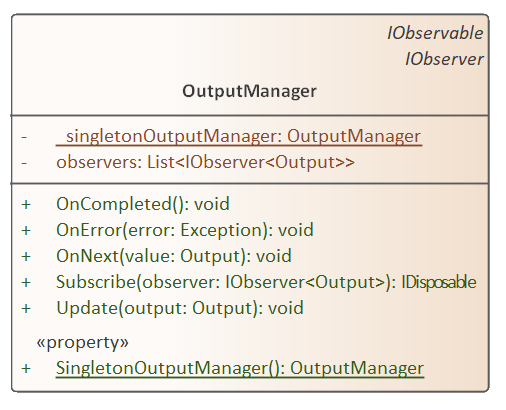
\includegraphics[scale=0.75]{../uml_klassen/StepDetectionLib/OutputManager.png}
    	\end{minipage}
    	\begin{minipage}{0.25\textwidth}	
        Gibt die berechneten Schrittdaten an Anwender weiter.
    	\end{minipage}
    	
        \paragraph{Properties:}
        \begin{itemize}
            \i{private static OutputManager singletonOutputManager} Enthält ein OutputManager-Objekt um das Singleton Entwurfsmuster zu implementieren.
            \i{private List<IObserver<Output>> observers} Liste der Beobachter.
            \i{public static OutputManager SingletonOutputManager} \glsnote{ro}
        \end{itemize}
        \paragraph{Methoden}
        \begin{itemize}
            \i{public void OnCompleted()} Wenn Subjekt fertig mit der Datenübertragung ist.
            \i{public void OnError(Exception error)} Wenn Subject einen Fehler erfährt.
            \i{public void OnNext(AccGyroData value)} Enthält Daten von Subjekt.
            \i{public IDisposable Subscribe(IObserver<Output> observer)} Fügt neue Beobachter hinzu.
            \i{public void Update(Output output)} Pusht Daten zu Beobachtern.
        \end{itemize}
    

    \subsection{Output}
    \sign{public struct Output}
    	\begin{minipage}{0.55\textwidth}
    		  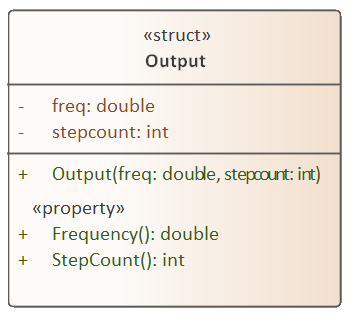
\includegraphics[scale=0.75]{../uml_klassen/StepDetectionLib/Output.png}
    	\end{minipage}
    	\begin{minipage}{0.45\textwidth}
    		Enthält double Schrittfrequenz und int Schrittanzahl und ist das Datenausgabeformat.
    	\end{minipage}
    	
        \paragraph{Properties:}
        \begin{itemize}
            \i{private double freq} Schrittfrequenz.
            \i{private int stepcount} Anzahl der Schritte.
            \i{public double Frequency} \glsnote{ro}
            \i{public int StepCount} \glsnote{ro}
        \end{itemize}
        \paragraph{Methoden}
        \begin{itemize}
            \i{public Output(double freq, int stepcount)} Konstruktor für Output.
        \end{itemize}


                        
\end{document}
